\section{Introduction}
\label{sec:intro}


Large language models have moved beyond academic benchmarks into systems that touch nearly every aspect of daily life except the physical world: not text on a screen but actions in a kitchen, a warehouse, or a hospital. Robots deployed in these settings face a long list of tasks that no fixed skill library can anticipate—folding laundry one moment, assembling parts the next, picking up after a child the moment after that. Kitchens, offices, labs, and factories each impose their own objects, layouts, and tolerances, and the policies that operate in them must generalize accordingly. The long-standing aspiration is therefore a single generalist controller—one model that transfers across tasks, scenes, and embodiments—rather than a fleet of task-specific policies hand-engineered one at a time.

This aspiration has driven the field toward vision–language–action (VLA) models, which build on vision–language model (VLM) backbones pre-trained on web-scale image–text data and are then trained on diverse robot trajectories to map pixels and language directly to actions. Progress over the past two years has been rapid, with successive generations of VLAs posting increasingly impressive task-success numbers on standardized benchmarks.

Yet despite this progress, current most VLAs fall short of this vision along several axes making them unfavorable for real-world deployments. 
(i) Frontier VLAs~\citep{team2024gemini,team2025gemini,rhoda2026dva,generalist2026gen1} are effectively closed systems: their training data, recipes, and model weights are proprietary. The few exceptions release weights alone, withholding the data and training procedures needed to reproduce or extend them. This opacity both impedes scientific progress and prevents practitioners from adapting these models to their own robots or fine-tuning on in-house demonstrations.
(ii) Recent systems~\citep{zhao2025cot,sun2024emma,lee2025molmoactactionreasoningmodels,zheng2024tracevla} have shown that explicit reasoning—chain-of-thought traces, predicted goal images, point trajectories, or full world-model rollouts—improves both action quality and the diagnosability of failures. In current implementations, however, this reasoning dominates inference latency: hundreds of tokens or entire predicted frames must be generated before a single action is emitted, and emerging world-model action models~\citep{kim2026cosmos,zhu2025unified} compound the problem with heavyweight per-step rollouts. The very mechanism intended to make policies more reliable thus renders them too slow for closed-loop control.
(iii) The few open-weights VLAs ~\citep{black2410pi0,intelligence2025pi05visionlanguageactionmodelopenworld} that can be run out-of-the-box are tied to expensive or specialized robot platforms beyond the reach of most academic labs and independent researchers. This constrains not only who can use these models, but also the diversity of settings in which they can be evaluated and improved.
(iv) Zero-shot performance remains brittle, and even after task-specific fine-tuning, success rates on realistic tasks fall well below the threshold required for dependable deployment.

\begin{figure}[t]
\centering
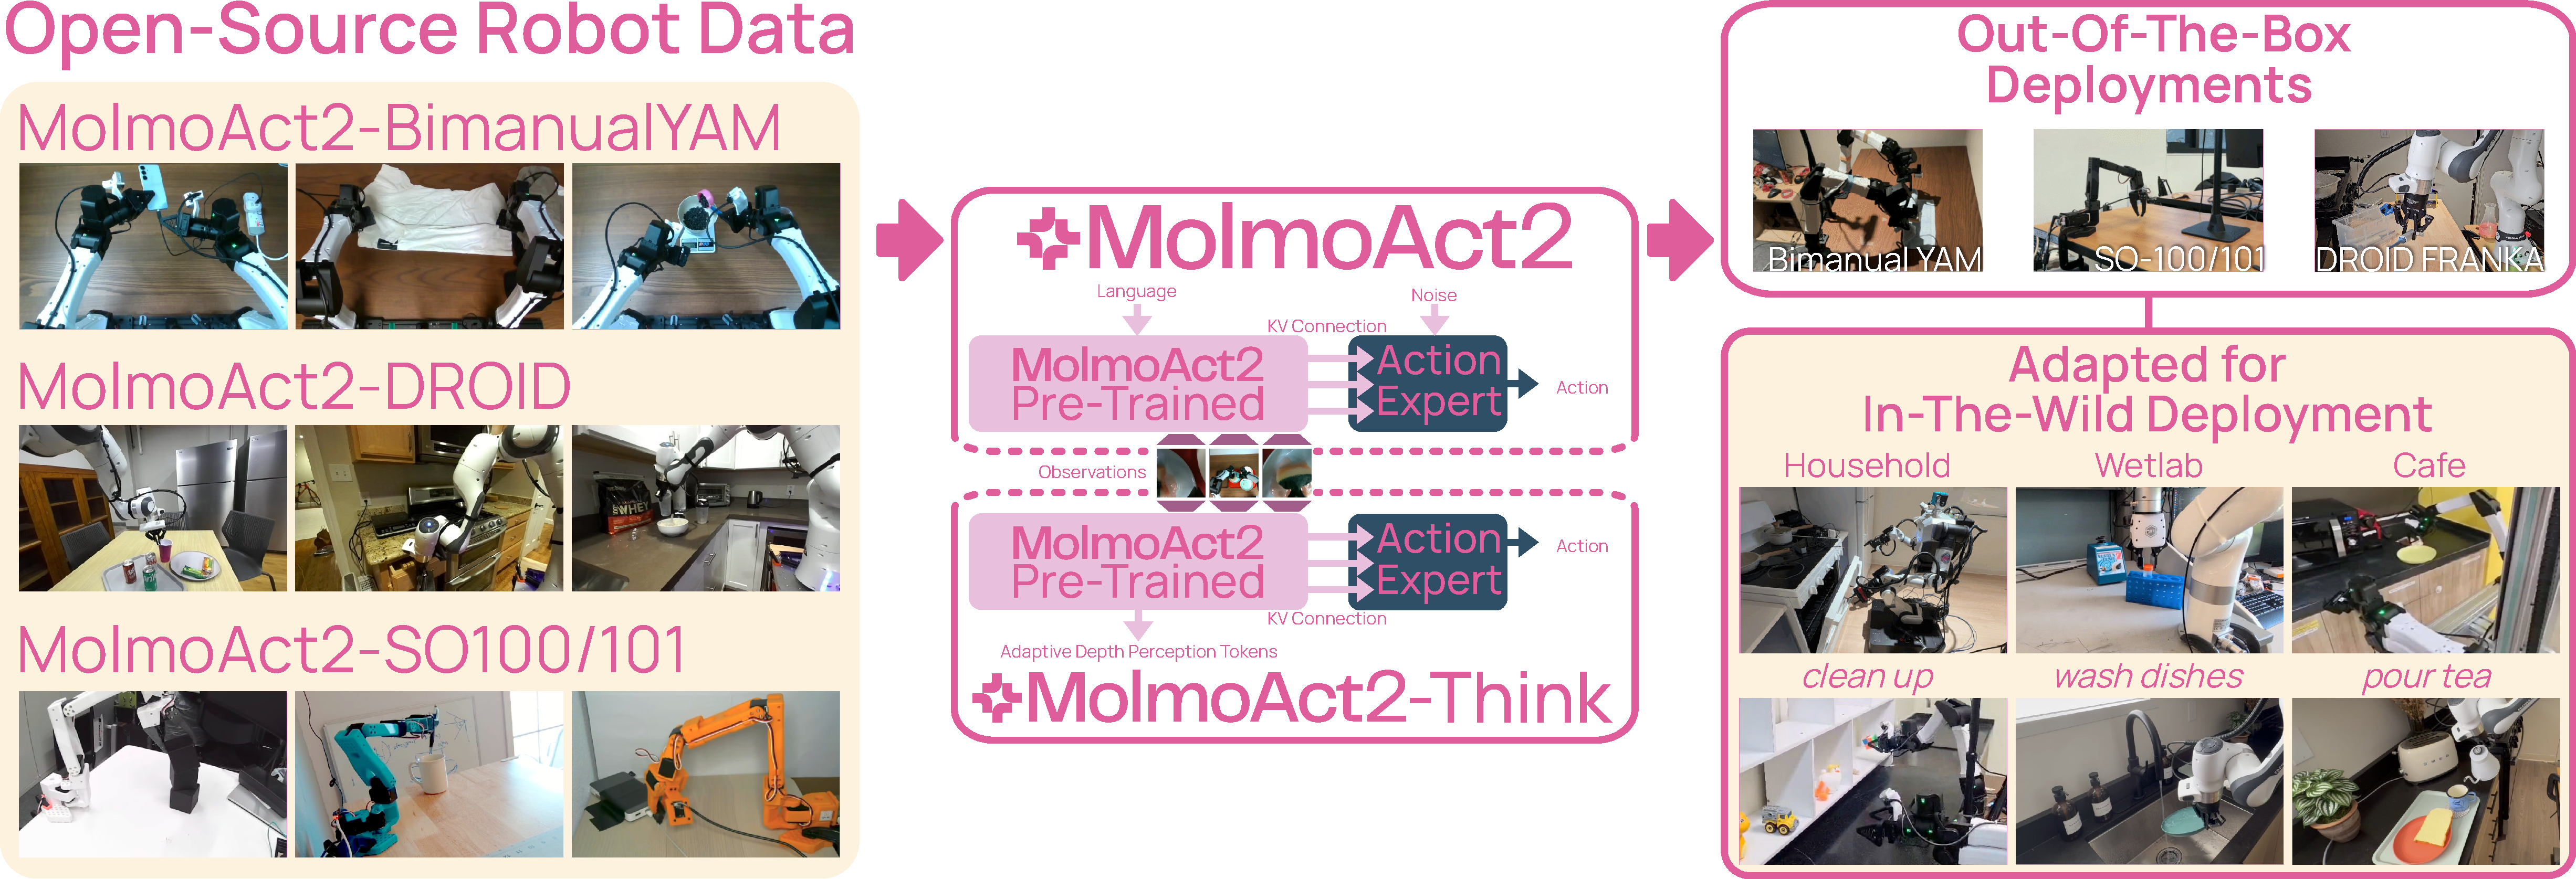
\includegraphics[width=\linewidth]{figures/MAF11.pdf}
\caption{\textbf{Overview of \molmoactt.} \molmoactt is a fully open action reasoning model for real-world deployment. From a suite of high-quality robot datasets that we collect, filter, and curate at scale across three platforms spanning the low-to-medium cost range (left), we train \molmoactt and its adaptive-depth reasoning variant \molmothink, coupled to the VLM backbone through per-layer KV conditioning (center). The resulting models deploy out-of-the-box on bimanual YAM, SO-100/101, and DROID Franka, and adapt to in-the-wild tasks such as cleaning up, washing dishes, wetlab automation, and pouring tea (right).}
\label{fig:teaser}
\end{figure}

In this paper, we present \molmoactt, an action reasoning model built for real-world deployment: fully open, deployable out-of-the-box on accessible embodiments, performant, and capable of fast, interpretable reasoning (Figure~\ref{fig:teaser}). \molmoactt improves over its predecessor MolmoAct~\citep{lee2025molmoactactionreasoningmodels} along five axes: a stronger embodied-reasoning VLM backbone, new training datasets, \molmoactfast, a redesigned VLA architecture, and a new reasoning paradigm.
General-purpose VLMs underspecify the embodied skills a policy needs—metric distances, free space, cross-view object tracking, and scene geometry. We address this with \molmoer (Sec.~\ref{sec:er}), a VLM specialized for spatial and embodied reasoning, initialized from Molmo2 and trained on a 3.3M-sample spatial–embodied corpus using a specialize-then-rehearse recipe. To support both pre-training and post-training of action models on top of this backbone, we release three datasets in Sec.~\ref{sec:data} targeting three platforms across the low-to-medium cost range: (i) \molmoacttyamdata, 720 hours of teleoperated YAM trajectories spanning tabletop and household tasks—the largest open bimanual dataset to date; (ii) \molmoacttsodata, a filtered subset of internet SO-100/101 data with mislabeled and low-quality trajectories removed; and (iii) \molmoacttdroiddata, a quality-filtered Franka subset of DROID. To make these trajectories usable under a discrete autoregressive objective, we introduce \molmoactfast, an open-weight, open-data implementation following FAST~\citep{pertsch2025fast}. We release its weights along with the millions of trajectories across five embodiments used to train it; \molmoactfast compresses one second of 32-D continuous actions into a compact discrete sequence. From the \molmoacttpre checkpoint, we then attach an action expert that generates continuous trajectories via flow matching and per-layer KV conditioning. Finally, we introduce \molmothink, the reasoning variant of \molmoactt, which performs adaptive depth reasoning by autoregressively predicting only the depth tokens for scene regions that change between timesteps. This exploits trajectory-level temporal redundancy to reduce latency proportional to the static scene fraction while retaining the geometric grounding that significantly improves model performance.

To understand the capabilities of \molmoactt and assess its readiness for real-world deployment, we conduct the most extensive empirical study of any open VLA to date, spanning 7 environment benchmarks across both simulation and the real world. Across all of them, \molmoactt and \molmothink outperform every strong baseline. We show that \molmoactt's fine-tuned checkpoints, \molmoacttdroid and \molmoacttso, can be deployed out of the box on their respective embodiments without any additional fine-tuning, significantly surpassing $\pi_{0.5}$~\citep{intelligence2025pi05visionlanguageactionmodelopenworld} (Sec.\ref{sec:exp-outbox}). We further demonstrate that \molmoactt is built on one of the strongest embodied-reasoning VLM backbones available: \molmoer surpasses models such as GPT-5~\citep{singh2025openai} and Gemini Robotics Embodied Reasoning (ER)-1.5~\citep{team2025gemini15} on 13 standard embodied-reasoning benchmarks (Sec.\ref{sec:exp-er}). For rapid real-world deployment via efficient fine-tuning to new embodiments, \molmoactt opens large performance gaps over strong general-purpose VLAs such as $\pi_{0.5}$~\citep{intelligence2025pi05visionlanguageactionmodelopenworld} not only on the two mainstream simulation benchmarks LIBERO~\citep{liu2023libero} and RoboEval~\citep{wang2025roboeval}, but also on a comprehensive evaluation suite of 8 real-world tasks on the bimanual YAM setup (Sec.\ref{sec:exp-ft}). Finally, our \molmothink models yield further gains over \molmoactt while providing additional interpretability that aids both diagnosis and performance (Sec.\ref{depth}).

\molmoactt is fully open in every respect, and beyond that, is capable of supporting real-world deployment for practical tasks: we release the model weights, training code, and the complete training dataset. We aim for \molmoactt to be more than an academic robotics foundation model; we want it to be a model that can be deployed in real-world workflows and deliver meaningful social impact.
